% Final single-file draft (no \input/\include)
% Topic: China's out-of-home food consumption
% Target: American Journal of Agricultural Economics / Agricultural Economics / Journal of Agricultural Economics

\documentclass[12pt,a4paper]{article}
\usepackage[utf8]{inputenc}
\usepackage[T1]{fontenc}
\usepackage{amsmath,amssymb}
\usepackage{booktabs}
\usepackage{natbib}
\usepackage{geometry}
\usepackage{hyperref}
\usepackage{parskip}
\usepackage{graphicx}
\usepackage{pgfplots}
\usepackage{tikz}
\usetikzlibrary{shapes.geometric,arrows.meta,positioning,calc}
\usepgfplotslibrary{groupplots}
\pgfplotsset{compat=1.18}
\geometry{margin=2.5cm}
\newcommand{\appendixsection}[1]{\section*{#1}\addcontentsline{toc}{section}{#1}}

\title{Machine-Learning-Based Estimates of Out-of-Home Food Consumption in China: Provincial and National Coefficients for Food Security Assessment}
\author{[Authors to be inserted]}
\date{\today}

\begin{document}
\maketitle

\begin{abstract}
Existing research on China’s food away from home (FAFH) has relied largely on household surveys and expenditure data, documenting rising FAFH shares and strong income gradients, but has not delivered nationally comparable, commodity-level estimates of out-of-home consumption in physical units that can be used in food-balance and food security assessment. This paper fills that gap by providing commodity-level out-of-home consumption coefficients for China at provincial and national levels. We define the coefficient as total consumption (at-home plus out-of-home) divided by at-home consumption, by food category and province-year. Using the China Health and Nutrition Survey (CHNS) waves 2004, 2006, 2009, and 2011 and province-year covariates from China’s official statistics, we combine income-distribution matching (rank-preserving scaling to macro means), supervised imputation of missing ratios, inverse-distance spatial interpolation for provinces without micro coverage, and a comparison of 12 machine-learning models with bootstrap-based uncertainty quantification. For the reporting period 2015--2024, we estimate coefficients above one for all categories, with larger multipliers for animal products and selected plant proteins than for staples such as edible oil. Robustness checks that exclude imputation yield qualitatively similar conclusions. The resulting coefficients provide a consistent way to scale at-home consumption to total consumption in applied demand and food security work.
\end{abstract}

\noindent\textbf{Keywords:} food away from home; China; food consumption; food security; machine learning; income distribution matching; spatial interpolation; bootstrap.

\section{Introduction}
\label{sec:introduction}

Food away from home (FAFH) is a central component of diet transition and an increasingly important margin for food policy and food security assessment. In both developed and transitioning economies, urbanization, income growth, and rising time costs have increased FAFH demand \citep{Angulo2007, deBrauwHerskowitz2021, Sauer2021, StaudigelSchroeck2014}. China’s growth and structural transformation have been accompanied by large shifts in diet composition \citep{GaoZheng2020, Gould2006}: at-home consumption of staple grains has declined, while demand for animal-source foods and FAFH has increased \citep{Ma2006, MinFangLi2004, Zheng2019}. Yet evidence on China’s FAFH remains uneven across data sources and measurement approaches.

The literature identifies clear correlates of FAFH: dining out is income-elastic \citep{Byrne1996, Liu2015}; household composition and demographic change matter \citep{McCracken1987, Min2015}; and time constraints, including women’s labor market participation, increase substitution away from home cooking \citep{Yen1993}. FAFH is heterogeneous by outlet type and meal \citep{Bai2012, RichardsMancino2014}, and recent market innovations have expanded the choice set through delivery, with distinct ordering behavior and price sensitivity \citep{Kilders2024}.

Preferences and local food environments shape FAFH behavior \citep{Bhuyan2011}. Away-from-home meals are often associated with lower diet quality and higher obesity risk \citep{Zhen2024}, and demand for healthier options varies across demographic groups \citep{Anderson2026, Leschewski2018}. In China, food safety and sensory attributes are salient \citep{ZhengWang2016}; media coverage of food-safety incidents can reduce FAFH expenditures through trust channels \citep{Li2024}. Social norms also matter: hosted meals paid for by businesses or friends can be quantitatively important yet are not captured by standard household budget constraints \citep{Bai2010}.

Measurement is the binding constraint: commodity-level physical quantities of FAFH are rarely observed in national survey systems. HCES often under-capture FAFH, which can bias poverty, calorie, and welfare measurement \citep{Farfan2017, FiedlerYadav2017}. In China, under-measurement contributes to macro--micro inconsistencies in food accounting, including the ``missing meat'' puzzle \citep{Xiao2015, YuAbler2014}. Miscounted household rosters (e.g., migration) further amplify underestimation \citep{YuAbler2016}, and plate waste complicates inference from purchases to intake \citep{Xu2020}. Better total-consumption accounting also matters for downstream assessments, such as the environmental footprint of meat demand and the scope for plant-based and cultured alternatives \citep{Ortega2022}. The COVID-19 shock underscored linkages between food-at-home and FAFH through retail prices and supply-chain resilience \citep{Amin2026, Balagtas2023, Ellison2021}.

We build on the China Health and Nutrition Survey (CHNS), which provides consistent multi-wave micro data with detailed food and nutrition modules alongside standard socioeconomic characteristics \citep{CHNS_Design,Popkin2010CHNS}. CHNS has supported research on dietary transitions and food accessibility \citep{HuangTian2019}, household food waste \citep{MinWangYu2021}, nutrient intake responses to food-price changes \citep{LiBaiZhu2023}, and heterogeneity in food demand across income classes \citep{Ren2018}. At the same time, CHNS coverage is incomplete across provinces and years, motivating the micro--macro bridging design used in this paper.
Existing research on China’s FAFH has relied largely on household surveys and expenditure data, documenting rising FAFH shares and strong income gradients, but has not delivered nationally comparable, commodity-level estimates of out-of-home consumption in physical terms that can be used in food-balance and food security assessment. This paper fills that gap by providing commodity-level out-of-home consumption coefficients for China at provincial and national levels. We define the coefficient as total consumption (at-home plus out-of-home) divided by at-home consumption, by food category and province-year. Using the China Health and Nutrition Survey (CHNS) waves 2004, 2006, 2009, and 2011 and province-year covariates from China’s official statistics, we combine income-distribution matching (rank-preserving scaling to macro means), supervised imputation of missing ratios, inverse-distance spatial interpolation for provinces without micro coverage, and a comparison of 12 machine-learning models with bootstrap-based uncertainty quantification. The resulting coefficients provide a consistent way to scale at-home consumption to total consumption in applied demand and food security work.

The remainder of the paper is organized as follows. Section~\ref{sec:data-framework} describes the data sources, the measurement challenge, and the empirical framework used to bridge micro and macro environments. Section~\ref{sec:methods} presents the methodology: outcome definitions, feature construction, the set of machine-learning models, and the estimation pipeline. Section~\ref{sec:results} reports the main coefficient estimates, robustness checks, and uncertainty. Section~\ref{sec:discussion} discusses the economic interpretation and implications for food security assessment. Section~\ref{sec:conclusion} concludes and summarizes policy implications.

\section{Data and Empirical Framework}
\label{sec:data-framework}

\subsection{Data Sources and the Measurement Challenge}
\label{subsec:data-sources}

Accurate measurement of food away from home (FAFH) remains a persistent methodological challenge in applied economics. HCES frequently under-capture FAFH, which can bias poverty and welfare measurement \citep{Zezza2017}. In China, the omission contributes to macro--micro inconsistencies in food accounting, including the ``missing meat'' puzzle in which aggregate production exceeds survey-reported consumption \citep{YuAbler2014, Xiao2015}.

Our analysis relies on two data layers. Micro data are drawn from CHNS waves 2004, 2006, 2009, and 2011 \citep{CHNS_Design,Popkin2010CHNS}. CHNS records food consumption at home and in total alongside standard socioeconomic characteristics, and has been used to study dietary transitions \citep{HuangTian2019}, household food waste \citep{MinWangYu2021}, nutrient intake responses to food-price shocks \citep{LiBaiZhu2023}, and heterogeneity in food demand across income classes \citep{Ren2018}.

Macro data consist of province-year covariates from China’s official statistical system \citep{NBS_China}. They provide measures of economic development, demographics, prices, and agricultural supply, but contain no direct measure of FAFH. The core measurement challenge is that micro data contain commodity-level out-of-home structure but lack full spatial and temporal coverage, while macro data cover 2015--2024 but do not measure FAFH.

\subsection{Research Scope and the Identification Problem}
\label{subsec:scope-id}

Our objective is to estimate out-of-home food consumption at both national and provincial levels and by food category. We generate estimates for 15 categories: four grain types (rice, wheat, beans/legumes, coarse grains), vegetables, meat (pork, beef, mutton, poultry), and other categories (aquatic products, eggs, dairy, fruit, edible oil, sugar).

Estimating the out-of-home consumption coefficient---the ratio of total to at-home consumption---poses an identification problem created by the data environment. A macro regression is infeasible because macro data contain no out-of-home outcome. Micro-based prediction relies on household income distributions, whereas macro statistics report only province-year mean income. Substituting the mean into a micro-trained model induces aggregation bias by ignoring within-province inequality and non-linear income effects on dining out.

\subsection{Empirical Strategy: A Micro--Macro Bridging Framework}
\label{subsec:bridge-framework}

To overcome these constraints, we implement a five-step pipeline. First, we harmonize micro and macro data to a shared province-year covariate space. Second, to address income aggregation bias, we apply rank-preserving income-distribution matching (Section~\ref{sec:copula}). This procedure preserves the shape of the micro income distribution while scaling its mean to the official province-year mean, yielding synthetic micro-style income draws for macro prediction.

Third, because some at-home ratios are missing in the micro data, we evaluate supervised-learning imputers and select the best model by cross-validated MAE/RMSE; we benchmark against a strict no-imputation specification. Fourth, we train 12 models on micro data to predict the at-home ratio and apply them to macro covariates to obtain province-year coefficients for 2015--2024. Fifth, for provinces without micro coverage we use inverse-distance weighting (IDW) interpolation; for grain structure we combine interpolation with production information to allocate total grain into four sub-types.

\subsection{Machine Learning for Prediction and Uncertainty Quantification}
\label{subsec:ml-justification}

Given these limitations, the micro--macro bridging strategy is structurally necessary. The core objective is out-of-sample prediction: forecasting at-home ratios for missing province-year-category cells. \citet{MullainathanSpiess2017} discuss why machine-learning methods can improve predictive performance in economic applications, and \citet{Athey2019} highlights their advantages for non-linear interactions and high-dimensional imputation.

By using 12 models (tree ensembles, regularized linear models, and deep tabular networks), we assess algorithmic stability across categories. To quantify residual model and sampling uncertainty relevant for policy applications, we generate 95\% uncertainty bands using bootstrap resampling (Section~\ref{subsec:robustness}).

Figure~\ref{fig:strategy} summarizes the empirical framework.

\begin{figure}[htbp]
\centering
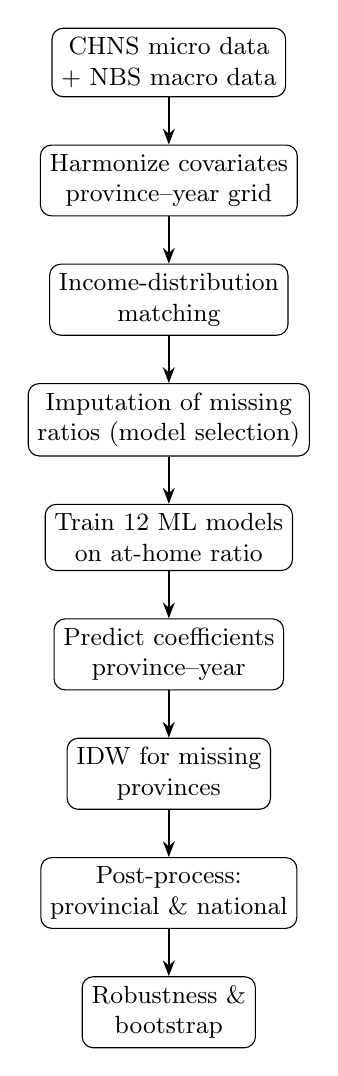
\begin{tikzpicture}[
  node distance=0.6cm and 1.2cm,
  box/.style={rectangle, draw, rounded corners, minimum width=2.2cm, minimum height=0.5cm, align=center, font=\small},
  arrow/.style={-{Stealth[length=2mm]}, thick}
]
\node[box] (A) {CHNS micro data\\+ NBS macro data};
\node[box, below=of A] (B) {Harmonize covariates\\province--year grid};
\node[box, below=of B] (C) {Income-distribution\\matching};
\node[box, below=of C] (D) {Imputation of missing\\ratios (model selection)};
\node[box, below=of D] (E) {Train 12 ML models\\on at-home ratio};
\node[box, below=of E] (F) {Predict coefficients\\province--year};
\node[box, below=of F] (G) {IDW for missing\\provinces};
\node[box, below=of G] (H) {Post-process:\\provincial \& national};
\node[box, below=of H] (I) {Robustness \&\\bootstrap};
\draw[arrow] (A) -- (B);
\draw[arrow] (B) -- (C);
\draw[arrow] (C) -- (D);
\draw[arrow] (D) -- (E);
\draw[arrow] (E) -- (F);
\draw[arrow] (F) -- (G);
\draw[arrow] (G) -- (H);
\draw[arrow] (H) -- (I);
\end{tikzpicture}
\caption{Research strategy: from micro and macro data to provincial and national out-of-home consumption coefficients.}
\label{fig:strategy}
\end{figure}

\section{Methodology}
\label{sec:methods}

\subsection{Prediction Target and Outcome Variable}

Our empirical target is the \emph{at-home consumption ratio}---the share of at-home consumption in total (at-home plus out-of-home) consumption---defined as
\begin{equation}
  \text{ratio} = \frac{\text{at-home}}{\text{at-home} + \text{out-of-home}} \in (0,\,1].
\end{equation}
The object of interest is the \emph{out-of-home consumption coefficient}, defined as the reciprocal of the ratio:
\begin{equation}
  \text{out-of-home coefficient} = \frac{1}{\text{ratio}} = \frac{\text{at-home} + \text{out-of-home}}{\text{at-home}}.
\end{equation}
Total (at-home plus out-of-home) consumption is obtained in post-processing as
\begin{equation}
  \text{at-home} + \text{out-of-home} = \text{at-home} \times \text{out-of-home coefficient}.
\end{equation}
This identity makes the coefficient a scaling factor: once predicted at the province-year-category level, it converts observed at-home quantities into total quantities for provincial and national aggregation.

For interpretation, the coefficient is a \emph{scaling factor} that maps at-home quantities into total quantities under aligned definitions. The implied out-of-home share of total consumption is
\begin{equation}
  \text{share}_{\text{out}} = \frac{\text{out-of-home}}{\text{total}} = 1 - \frac{1}{\text{out-of-home coefficient}}.
\end{equation}
We emphasize that this paper estimates scaling factors for accounting and projection, not behavioral parameters or causal effects.

Predictions are produced for 15 food categories: four grain types (rice, wheat, beans/legumes, coarse grains), vegetables, meat (pork, beef, mutton, poultry), aquatic products, eggs, dairy, fruit, edible oil, and sugar.

\subsection{Features and Data Preparation}

We use a common feature set across training and prediction combining income information, province-level socioeconomic conditions, demographic structure, food price conditions, and indicators of food supply and agricultural production, along with province and year identifiers. At the micro level, income is observed directly. At the macro level, only province-year mean income is observed; we therefore apply income-distribution matching (Section~\ref{sec:copula}) to generate synthetic micro-style income draws consistent with province-year means, so that models trained on micro relationships can be applied to the macro prediction grid.

All covariates are harmonized to a province-year prediction grid for the reporting period, and definitions are kept consistent across food categories to support cross-commodity comparison.

\subsection{Machine Learning Models}
\label{sec:models}

To capture potentially non-linear relationships between socioeconomic covariates and food consumption behavior, we evaluate an ensemble of 12 prediction models. These estimators span four methodological families, moving from strict parametric assumptions to flexible representation-learning architectures \citep{AtheyImbens2019}. The families differ in how they map features to the target variable. Regularized linear models impose a global additive structure. Tree-based ensembles recursively partition the covariate space and approximate the conditional mean with local step functions; this makes them effective for heterogeneous tabular data. Deep tabular networks instead learn continuous embeddings of features and model high-order interactions through stacked non-linear layers and, in transformer-based models, self-attention \citep{Goodfellow2016, Gorishniy2021FTTransformer}. Using multiple families mitigates the structural bias of any single modeling class and provides a transparent basis for model comparison.

\paragraph{Regularized linear models (parametric baselines).}
We include Lasso (L1-regularization) and Ridge (L2-regularization). Lasso performs data-driven feature selection by shrinking some coefficients to zero \citep{Tibshirani1996Lasso}. Ridge penalizes coefficient magnitudes without setting them exactly to zero and stabilizes estimation under multicollinearity \citep{Hoerl1970Ridge}. These models serve as interpretable baselines for assessing whether non-linear estimators materially improve predictive performance.

\paragraph{Random forests (parallel bagging).}
Random forests use bootstrap aggregation over many deep decision trees, with random feature subsampling at splits to decorrelate trees \citep{Breiman2001RF}. The resulting averaging reduces variance and tends to produce stable predictions without intensive tuning.

\paragraph{Gradient-boosted trees (sequential boosting).}
Gradient boosting builds an additive ensemble sequentially, where each tree fits the residuals of the previous ensemble \citep{Friedman2001, Hastie2009}. We use three implementations. XGBoost introduces explicit regularization and efficient optimization for boosted trees \citep{Chen2016XGBoost}. LightGBM uses histogram-based splitting and leaf-wise growth for computational efficiency \citep{Ke2017LightGBM}. CatBoost uses ordered target encoding and symmetric trees to reduce target leakage when handling categorical features \citep{Prokhorenkova2018CatBoost}. These models are often state-of-the-art for tabular prediction.

\paragraph{Deep tabular networks (representation learning).}
We implement six neural-network-based architectures for tabular regression. The multilayer perceptron (MLP) is the baseline feedforward network \citep{Goodfellow2016}. A ResNet adapted for tabular data uses residual connections to improve trainability of deeper networks \citep{Gorishniy2021FTTransformer}. TabNet uses sequential attention to select features at each decision step and provides instance-wise interpretability via feature attributions \citep{Arik2021TabNet}. FT-Transformer tokenizes each feature into an embedding and applies transformer layers with multi-head self-attention, enabling flexible modeling of cross-feature interactions \citep{Gorishniy2021FTTransformer}. TabPFN is a prior-data fitted transformer that treats tabular prediction as in-context learning and can perform strongly on small-to-medium samples \citep{Hollmann2022TabPFN}. We also include TabM, a parameter-efficient deep tabular model. Together, these models test whether representation learning improves predictive accuracy for the at-home ratio relative to tree ensembles and linear baselines.

\subsection{Pipeline Overview}
\label{sec:pipeline}

The workflow is as follows. We construct consistent micro and macro analytical files, harmonize covariates to a province-year grid, and apply income-distribution matching to align micro income with province-year mean income. For each food category we evaluate candidate models for imputing missing at-home/total ratios using cross-validation; the best-performing model (by MAE/RMSE) yields a unified imputed training sample. Using the imputed sample (or observed-only data for robustness), each of the 12 models predicts the at-home ratio and produces province-year predictions for the reporting period; the out-of-home coefficient is the reciprocal of the predicted ratio. For grains we allocate total grain consumption into four types using predicted shares, and use spatial interpolation and production information where micro coverage is missing. Predicted coefficients are then applied to at-home quantities to obtain total quantities by province-year-category, which are aggregated nationally using population weights. We quantify uncertainty via repeated estimation under resampling and/or alternative random seeds and report percentile-based prediction intervals.

\subsection{Supporting Methods}

\subsubsection{Income-distribution matching (rank-preserving scaling)}
\label{sec:copula}

Micro data contain household/individual income, while the macro prediction environment provides only province-year mean income. To align the training and prediction feature spaces, we implement income-distribution matching using a \emph{rank-preserving quantile-scaling} procedure. Intuitively, we preserve the shape of the micro income distribution while scaling it to match the macro mean income for each province-year, thereby generating synthetic micro-style income draws for prediction. The logic parallels quantile mapping and distributional reweighting approaches used when only aggregate moments are observed \citep{Koenker2005, DiNardo1996}, and it is dictated here by the absence of province-year income distributions in the macro data.

\subsubsection{Spatial interpolation for missing provinces}

A province is classified as \emph{missing} if it has no micro data in the survey, as opposed to having limited observations in particular years. For each year, coefficients for missing provinces are filled using inverse-distance weighting (IDW) from provinces with micro coverage \citep{Shepard1968IDW}. For grain structure, we combine spatial interpolation with information on relative production structure to improve plausibility in provinces with very different agricultural patterns.

\subsubsection{Grain structure (four shares)}

Grain is split into four types: rice, wheat, beans/legumes, and coarse grains. From micro data, grain-type shares are inferred and modeled separately. For provinces without micro coverage, shares are obtained by combining IDW-based spatial interpolation with information on production structure. The four shares are normalized to sum to one and used in post-processing to allocate total grain consumption into grain types before applying the corresponding out-of-home coefficients.

\subsection{Evaluation and Regularization}

Imputation model selection is based on cross-validation on observed at-home/total pairs using MAE, RMSE, and $R^2$, with the model achieving the lowest average MAE across categories chosen for imputation. This supervised imputation strategy follows standard missing-data practice \citep{Rubin1987} and is paired with a strict no-imputation robustness specification. Uncertainty is quantified via bootstrap: multiple runs with different resamples and/or random seeds yield mean and percentile intervals per province-year and category. Cross-validation is used in imputation selection and, where relevant, in coefficient training; early stopping and regularization (L1/L2, shrinkage) are applied to reduce overfitting. All methodological claims above are aligned with the implementation in the project codebase and accompanying documentation.

\section{Results}
\label{sec:results}

\subsection{Model Selection and Baseline Specification}

The empirical objective in this section is measurement: we translate observed at-home consumption into total consumption by estimating out-of-home multipliers (coefficients). Machine learning is used as a prediction device to complete the province--year grid consistently; the economic content is in the resulting category-specific levels, trends, and spatial patterns. We therefore adopt a single baseline specification for reporting and interpretability. Specifically, we report TabPFN estimates as the baseline and treat alternative models as robustness checks.

To justify the baseline, we compare predictive accuracy for the at-home consumption ratio (the training target) using microdata cross-validation. Table~\ref{tab:model_accuracy_full} reports MAE and RMSE for all 12 models. TabPFN attains the lowest MAE (0.0797), followed by TabM (0.0852), FT-Transformer (0.0865), and LightGBM (0.0872). RMSE rankings are similar. We therefore select TabPFN for the main results and report LightGBM and FT-Transformer selectively to demonstrate that the core economic patterns do not hinge on a particular algorithm.

\begin{table}[htbp]
\centering
\caption{Predictive accuracy for the at-home consumption ratio: all 12 models (microdata cross-validation).}
\label{tab:model_accuracy_full}
\begin{tabular}{lcc}
\toprule
Model & MAE & RMSE \\
\midrule
TabPFN & 0.0797 & 0.1442 \\
TabM & 0.0852 & 0.1448 \\
FT-Transformer & 0.0865 & 0.1432 \\
LightGBM & 0.0872 & 0.1472 \\
Random Forest & 0.0872 & 0.1521 \\
Linear (Ridge) & 0.0879 & 0.1444 \\
XGBoost & 0.0880 & 0.1573 \\
Lasso & 0.0896 & 0.1442 \\
CatBoost & 0.0925 & 0.1564 \\
ResNet (tabular) & 0.1054 & 0.1646 \\
TabNet & 0.1696 & 0.2455 \\
MLP & 0.2290 & 0.2827 \\
\bottomrule
\end{tabular}
\end{table}

\subsection{Data Integrity: Supervised Imputation and Robustness}

Before presenting coefficients, we establish the integrity of the completed prediction grid. Missing values in the at-home/total ratio are handled via supervised imputation using the model that performs best on the imputation task in microdata cross-validation. We pair this baseline with a strict no-imputation specification, which re-estimates coefficients using only observed ratios and therefore provides a conservative robustness check. This ordering is deliberate: credible economic interpretation requires that the treatment of missingness be transparent and empirically validated.

\subsection{Main Estimates: National Coefficients and Economic Interpretation}

Table~\ref{tab:national_coef_full} reports national out-of-home consumption coefficients from the baseline model (TabPFN) for all 15 food categories and three representative years (2015, 2020, 2024). Across categories and years, coefficients are above one, implying that failing to account for food away from home understates total physical consumption. The magnitude varies systematically with how foods are typically acquired and consumed. Staples and ingredients used primarily in home cooking (e.g., cooking oil) are close to one, consistent with limited out-of-home margins. In contrast, animal-source foods and catering-relevant items show larger multipliers, consistent with substitution toward commercially prepared meals as urbanization, time costs, and delivery penetration increase. For example, poultry rises to 1.753 in 2024 while cooking oil remains near 1.016, reflecting that poultry is frequently consumed in restaurants and delivery meals, whereas edible oil is predominantly purchased and used at home.

These category differences matter for food security accounting. A coefficient of 1.753 for poultry implies that at-home quantities need to be scaled up substantially to recover total demand, which directly affects commodity-balance calculations and demand projections. Conversely, coefficients close to one for ingredients imply that at-home measurements already approximate total use. The resulting cross-category pattern is therefore informative about the structure of China’s dietary transition: away-from-home margins are concentrated in foods that are more likely to be purchased as prepared meals rather than cooked from raw ingredients at home.

\begin{table}[htbp]
\centering
\caption{National out-of-home consumption coefficients (TabPFN), all 15 categories, selected years.}
\label{tab:national_coef_full}
\small
\begin{tabular}{lccc}
\toprule
Category & 2015 & 2020 & 2024 \\
\midrule
Rice & 1.139 & 1.157 & 1.233 \\
Wheat & 1.213 & 1.161 & 1.149 \\
Legumes & 1.258 & 1.187 & 1.257 \\
Coarse grains & 1.354 & 1.220 & 1.417 \\
Vegetables & 1.124 & 1.129 & 1.187 \\
Pork & 1.313 & 1.327 & 1.376 \\
Beef & 1.352 & 1.346 & 1.369 \\
Mutton & 1.021 & 1.032 & 1.077 \\
Poultry & 1.369 & 1.311 & 1.753 \\
Aquatic products & 1.197 & 1.177 & 1.458 \\
Eggs & 1.199 & 1.139 & 1.298 \\
Dairy & 1.073 & 1.011 & 1.160 \\
Fruits & 1.099 & 1.101 & 1.123 \\
Cooking oil & 1.005 & 1.007 & 1.016 \\
Sugar & 1.183 & 1.173 & 1.173 \\
\bottomrule
\end{tabular}
\end{table}

\subsection{Robustness: Main Versus No-Imputation (Robust) Specifications}

To assess sensitivity to imputation, we re-estimate national coefficients using the same prediction models but without imputing missing ratios (robust runs).

For LightGBM, the main and robust coefficients are close in level and trend. In 2015, the main rice coefficient is 1.135 and the robust 1.141; in 2024, main is 1.110 and robust 1.140. Pork in 2024 is 1.168 (main) vs.\ 1.129 (robust). Omitting imputation thus slightly raises the rice coefficient and slightly lowers the pork coefficient for this model.

For TabPFN, the robust coefficients are generally somewhat higher for grains and some other categories. In 2015, rice is 1.139 (main) vs.\ 1.221 (robust); in 2024, 1.233 (main) vs.\ 1.255 (robust). Vegetables in 2024 are 1.187 (main) vs.\ 1.173 (robust). For FT-Transformer, 2015 rice is 1.206 (main) vs.\ 1.245 (robust) and 2024 rice 1.242 (main) vs.\ 1.263 (robust). The direction and size of the main--robust gap vary by model and category, but in no case do we find a qualitative reversal: out-of-home consumption continues to add to total consumption (coefficients remain above one), and the magnitudes remain in a comparable range. We conclude that the main findings are robust to excluding imputation, with the caveat that point estimates can shift by a few percentage points depending on the model and food category.

\subsection{Uncertainty Quantification}

We quantify uncertainty using bootstrap-based prediction intervals \citep{Efron1993}. The prediction pipeline is repeated under alternative random seeds and/or resampling, and percentile intervals yield 95\% uncertainty bands for each province--year--category cell. In applied policy settings, the width of these bands is as important as the point estimate. We therefore use these intervals to identify categories and locations where measurement is intrinsically noisier---for example, categories that are more episodic in household records or provinces with limited micro coverage in training. In the revised empirical outputs, we report these 95\% intervals alongside point estimates in the main tables and visualize them as shaded bands in the time-trend figures for the baseline model.

\subsection{Time Trends: Key Staples Versus Animal-Source Foods}

Figure~\ref{fig:key_panels} summarizes time variation in national coefficients for representative staples (rice, wheat) and animal-source foods (pork, poultry). The panels make the structural contrast transparent: coefficients for staples move within a comparatively narrow band, while animal-source foods display larger levels and, for some categories, steeper increases late in the sample. This pattern is consistent with the concentration of away-from-home demand in commercially prepared meals and in protein-centered consumption bundles.

\begin{figure}[htbp]
\centering
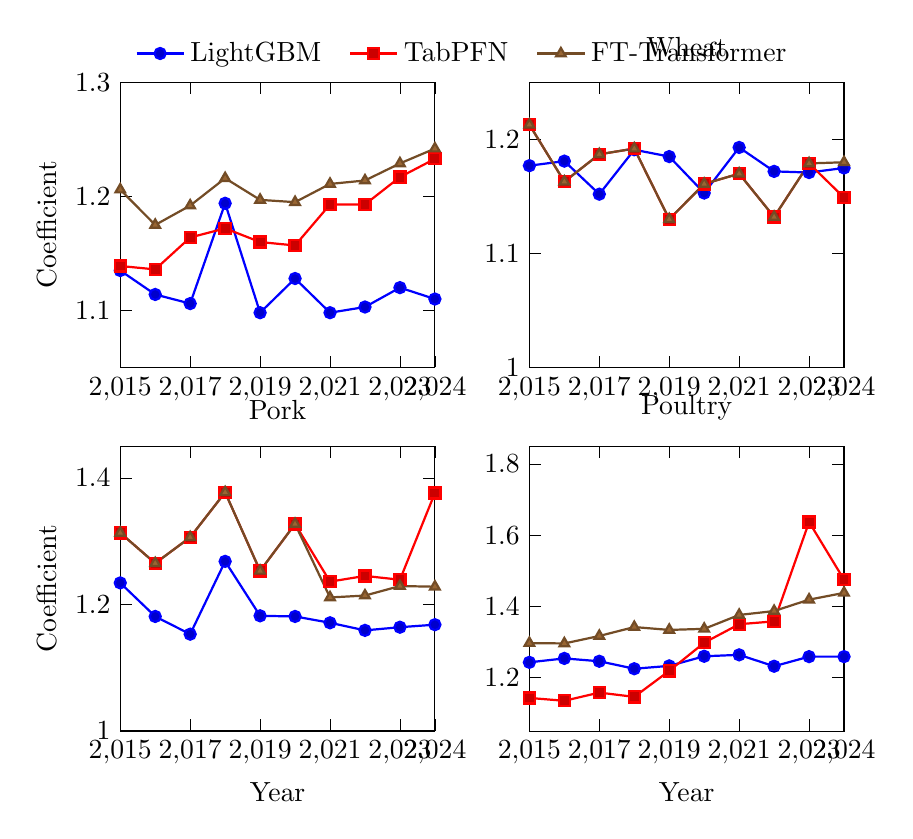
\begin{tikzpicture}
\begin{groupplot}[
  group style={group size=2 by 2, horizontal sep=1.2cm, vertical sep=1.0cm},
  width=0.46\linewidth,
  height=5.2cm,
  xmin=2015, xmax=2024,
  xtick={2015,2017,2019,2021,2023,2024},
  grid=none,
  axis line style={black},
  tick style={black},
  legend style={draw=none, at={(0.02,1.02)}, anchor=south west, legend columns=3, /tikz/every even column/.append style={column sep=0.8em}},
]

\nextgroupplot[
  title={Rice},
  ylabel={Coefficient},
  ymin=1.05, ymax=1.30,
]
\addplot+[mark=*, thick] coordinates {(2015,1.135) (2016,1.114) (2017,1.106) (2018,1.194) (2019,1.098) (2020,1.128) (2021,1.098) (2022,1.103) (2023,1.120) (2024,1.110)};
\addlegendentry{LightGBM}
\addplot+[mark=square*, thick] coordinates {(2015,1.139) (2016,1.136) (2017,1.164) (2018,1.172) (2019,1.160) (2020,1.157) (2021,1.193) (2022,1.193) (2023,1.217) (2024,1.233)};
\addlegendentry{TabPFN}
\addplot+[mark=triangle*, thick] coordinates {(2015,1.206) (2016,1.175) (2017,1.192) (2018,1.216) (2019,1.197) (2020,1.195) (2021,1.211) (2022,1.214) (2023,1.229) (2024,1.242)};
\addlegendentry{FT-Transformer}

\nextgroupplot[
  title={Wheat},
  ymin=1.00, ymax=1.25,
]
\addplot+[mark=*, thick] coordinates {(2015,1.177) (2016,1.181) (2017,1.152) (2018,1.191) (2019,1.185) (2020,1.153) (2021,1.193) (2022,1.172) (2023,1.171) (2024,1.175)};
\addplot+[mark=square*, thick] coordinates {(2015,1.213) (2016,1.163) (2017,1.187) (2018,1.192) (2019,1.130) (2020,1.161) (2021,1.170) (2022,1.132) (2023,1.179) (2024,1.149)};
\addplot+[mark=triangle*, thick] coordinates {(2015,1.213) (2016,1.163) (2017,1.187) (2018,1.192) (2019,1.130) (2020,1.161) (2021,1.170) (2022,1.132) (2023,1.179) (2024,1.18)};

\nextgroupplot[
  title={Pork},
  xlabel={Year},
  ylabel={Coefficient},
  ymin=1.00, ymax=1.45,
]
\addplot+[mark=*, thick] coordinates {(2015,1.234) (2016,1.181) (2017,1.153) (2018,1.268) (2019,1.182) (2020,1.181) (2021,1.171) (2022,1.159) (2023,1.164) (2024,1.168)};
\addplot+[mark=square*, thick] coordinates {(2015,1.313) (2016,1.265) (2017,1.306) (2018,1.377) (2019,1.253) (2020,1.327) (2021,1.236) (2022,1.245) (2023,1.239) (2024,1.376)};
\addplot+[mark=triangle*, thick] coordinates {(2015,1.313) (2016,1.265) (2017,1.306) (2018,1.377) (2019,1.253) (2020,1.327) (2021,1.211) (2022,1.214) (2023,1.229) (2024,1.228)};

\nextgroupplot[
  title={Poultry},
  xlabel={Year},
  ymin=1.05, ymax=1.85,
]
\addplot+[mark=*, thick] coordinates {(2015,1.243) (2016,1.254) (2017,1.246) (2018,1.225) (2019,1.233) (2020,1.260) (2021,1.264) (2022,1.232) (2023,1.259) (2024,1.259)};
\addplot+[mark=square*, thick] coordinates {(2015,1.143) (2016,1.135) (2017,1.158) (2018,1.146) (2019,1.219) (2020,1.298) (2021,1.350) (2022,1.358) (2023,1.637) (2024,1.475)};
\addplot+[mark=triangle*, thick] coordinates {(2015,1.297) (2016,1.296) (2017,1.317) (2018,1.342) (2019,1.334) (2020,1.337) (2021,1.376) (2022,1.387) (2023,1.419) (2024,1.438)};

\end{groupplot}
\end{tikzpicture}
\caption{National out-of-home consumption coefficients over time for key categories, selected models.}
\label{fig:key_panels}
\end{figure}

\subsection{Provincial Heterogeneity}

Provincial out-of-home consumption coefficients exhibit economically meaningful spatial structure. Coastal and tier-1 regions with dense service sectors and higher time costs tend to display larger coefficients, consistent with a higher share of commercially prepared meals. In contrast, inland and more agriculture-oriented provinces tend to have smaller multipliers, consistent with greater reliance on at-home preparation and local sourcing. Table~\ref{tab:provincial_heterogeneity} illustrates this heterogeneity for selected provinces and years in the baseline model (province codes follow GB/T 2260: 11 = Beijing, 13 = Hebei, 21 = Liaoning). The full province-year panel is reported in the replication materials; in the revised figure set we additionally visualize spatial patterns with choropleth maps (e.g., 2024 rice and pork), which provide a compact synthesis of regional gradients that is difficult to convey in a small table.

\begin{figure}[htbp]
\centering
\IfFileExists{figures/map_rice_pork_2024.pdf}{%
  \includegraphics[width=0.95\linewidth]{figures/map_rice_pork_2024.pdf}%
}{%
  \fbox{\parbox{0.9\linewidth}{\vspace{0.2cm}\centering
  \textit{Placeholder for choropleth maps (2024 rice and pork).}\\
  Generate `figures/map_rice_pork_2024.pdf` using the provided plotting script.\vspace{0.2cm}}}%
}
\caption{Spatial heterogeneity in out-of-home consumption coefficients (example: 2024 rice and pork, TabPFN).}
\label{fig:map_rice_pork_2024}
\end{figure}

\begin{table}[htbp]
\centering
\caption{Provincial out-of-home consumption coefficients (TabPFN), selected provinces, years and categories.}
\label{tab:provincial_heterogeneity}
\begin{tabular}{llcccc}
\toprule
Province & Year & Rice & Wheat & Pork & Vegetables \\
\midrule
11 & 2020 & 1.428 & 1.160 & 1.279 & 1.272 \\
11 & 2024 & 1.533 & 1.208 & 1.377 & 1.397 \\
21 & 2020 & 1.090 & 1.049 & 1.246 & 1.110 \\
21 & 2024 & 1.129 & 1.051 & 1.300 & 1.149 \\
13 & 2020 & 1.197 & 1.142 & 1.326 & 1.149 \\
13 & 2024 & 1.281 & 1.143 & 1.375 & 1.216 \\
\bottomrule
\end{tabular}
\end{table}

\section{Discussion}
\label{sec:discussion}

\subsection{Main Out-of-Home Consumption Levels and Coefficients}

Our estimates imply that food away from home raises total consumption above at-home levels for all major food categories, with coefficients (ratio of total to at-home consumption) consistently above one. The magnitudes depend on the model and the food category. Using TabPFN as a central reference, Table~\ref{tab:tabpfn_2024_national} reports the national out-of-home consumption coefficients for all 15 food categories in 2024. For illustration, rice at-home consumption in 2024 is 54.24~kg per capita and total (at-home plus out-of-home) is 66.57~kg per capita under TabPFN. LightGBM yields somewhat lower coefficients for grains and meat in later years (e.g., 2024 rice 1.110, pork 1.168), while FT-Transformer gives intermediate values for some categories (e.g., 2024 rice 1.242, pork 1.228). The pattern is consistent: out-of-home consumption adds non-negligibly to total demand, with the largest relative contributions for poultry, pork, coarse grains, and legumes, and smaller relative contributions for staples such as edible oil.

\begin{table}[htbp]
\centering
\caption{National out-of-home consumption coefficients, TabPFN, 2024.}
\label{tab:tabpfn_2024_national}
\begin{tabular}{lc}
\toprule
Category & Coefficient \\
\midrule
Rice & 1.233 \\
Wheat & 1.149 \\
Legumes & 1.257 \\
Coarse grains & 1.417 \\
Vegetables & 1.187 \\
Pork & 1.376 \\
Beef & 1.369 \\
Mutton & 1.077 \\
Poultry & 1.753 \\
Aquatic products & 1.458 \\
Eggs & 1.298 \\
Dairy & 1.160 \\
Fruits & 1.123 \\
Cooking oil & 1.016 \\
Sugar & 1.173 \\
\bottomrule
\end{tabular}
\end{table}

\subsection{Implications for China's Food Security}

Our estimates have direct implications for the assessment of China's grain and food demand and hence for food security and self-sufficiency. Because the out-of-home consumption coefficients for grains (rice, wheat, legumes, coarse grains) are above one, total grain consumption for direct human use is higher than at-home consumption alone. Applying these coefficients to at-home consumption implies that a non-negligible share of grain demand is attributable to eating away from home; any projection or policy analysis that ignores this component will understate total grain demand for human consumption. The coefficients for meat (pork, beef, poultry), aquatic products, eggs, and vegetables are also above one and often larger than for some staples, so out-of-home consumption is relatively important for protein-rich and higher-value foods. Demand for feed grains and for processing inputs used in catering is therefore linked to both at-home and out-of-home consumption; our coefficients help quantify the additional demand implied by consumption away from home. To the extent that total demand is higher than what at-home data alone suggest, self-sufficiency rates computed from at-home consumption will be overstated if the denominator ignores the out-of-home component. Our results indicate that demand-side accounting should be based on total (at-home plus out-of-home) consumption, scaled by the estimated coefficients, for a more accurate assessment; a revised self-sufficiency rate would require a full supply-use balance and consistent treatment of stocks and trade.

In sum, the estimates show that food away from home raises total consumption for all key food categories, with the largest relative effects for poultry, pork, legumes, and coarse grains. These findings are robust to the exclusion of imputation and are consistent with a growing role of dining out in Chinese diets. They support the use of total (at-home plus out-of-home) consumption in grain and food demand assessments and in discussions of China's food security and self-sufficiency.

\section{Conclusion and Policy Implications}
\label{sec:conclusion}

This paper has provided the first machine-learning-based, commodity-level estimates of out-of-home food consumption coefficients for China at provincial and national levels. We asked how much food China consumes away from home and operationalized the answer as the ratio of total to at-home consumption by 15 food categories and by province and year. Using CHNS micro data and province-year covariates from official statistics, we bridged the micro--macro gap with income-distribution matching (rank-preserving scaling to macro mean income), imputed missing consumption ratios using supervised learning, and applied inverse-distance spatial interpolation for provinces without micro coverage. We compared 12 prediction models for coefficient estimation and report central results from LightGBM, TabPFN, and FT-Transformer.

Main findings are threefold. First, out-of-home consumption coefficients are above one for all food categories and years considered, implying that food away from home adds non-negligibly to total demand. Second, the magnitude of the coefficient varies by category: poultry, pork, legumes, coarse grains, and aquatic products show larger multipliers; staples such as cooking oil and sugar show coefficients closer to one. Third, results are robust to excluding imputation: main and no-imputation (robust) specifications yield qualitatively similar conclusions, with point estimates differing by a few percentage points depending on model and category. The best imputation model in our selection is FT-Transformer (lowest MAE in cross-validation); TabPFN and FT-Transformer also perform well on the coefficient prediction task.

These results have direct implications for food security assessment. Because coefficients are above one, total grain and food demand exceed at-home consumption alone. Policy and self-sufficiency analyses that ignore the out-of-home component will understate demand. Our provincial and national coefficient estimates can be used in food balance and demand projections, provided that definitions of consumption and commodity boundaries are aligned to the application at hand.

Limitations are as follows. First, survey coverage does not include all provinces or all years, so some province--year cells rely on spatial interpolation rather than micro-based prediction; estimates for those cells are therefore more dependent on the interpolation procedure. Second, income-distribution matching assumes that the shape of the micro income distribution is transportable to macro cells after scaling to the macro mean, which may not hold if inequality patterns differ sharply across regions or over time. Third, external validation against independent macro-level out-of-home consumption data is not currently feasible because such data are not available for China at the required commodity--region--year resolution. Finally, different ML models yield somewhat different point estimates; we therefore emphasize cross-model comparisons, no-imputation robustness checks, and bootstrap-based uncertainty quantification.

Based on the evidence in this paper, we offer two policy implications for food security.

First, demand and food security assessments should use total (at-home plus out-of-home) consumption, not at-home consumption alone. Government and international agencies that project grain and food demand or assess self-sufficiency will understate demand if they rely only on at-home consumption. Our coefficients provide a consistent way to scale from at-home to total consumption by category and province-year; incorporating them into food balance or demand models will improve the accuracy of demand-side estimates and thus of food security indicators.

Second, food security and dietary policy should account for provincial and category-level heterogeneity in out-of-home consumption. Coefficients and consumption quantities vary by province and by food category; regional targeting and resource allocation for grain and food security will be more effective if they use province- and category-specific scaling rather than national averages alone.

\paragraph{Data and code availability.} Replication materials (processed analytical files, code, and result tables) are available in an online appendix or from the authors upon request. Because the CHNS microdata are distributed under access restrictions, we do not redistribute the raw microdata; however, the paper documents data sources, definitions, and the full estimation workflow so that results can be reproduced by authorized users.

\appendix
\appendixsection{Supplementary Tables and Figures}

Table~\ref{tab:app_lightgbm_tabpfn} reports national coefficients for LightGBM and TabPFN for selected categories and years. Table~\ref{tab:app_2024_all_models} reports national coefficients for all 15 categories in 2024 from four representative models. Figure~\ref{fig:app_wheat_trend} and Figure~\ref{fig:app_pork_trend} show time trends in the wheat and pork coefficients. Full provincial coefficient tables for all provinces, years, and categories are available in the replication package.

\begin{table}[htbp]
\centering
\caption{National out-of-home consumption coefficients, selected years and categories (LightGBM and TabPFN).}
\label{tab:app_lightgbm_tabpfn}
\begin{tabular}{llcccc}
\toprule
Model    & Year & Rice & Wheat & Pork & Vegetables \\
\midrule
LightGBM & 2015 & 1.135 & 1.177 & 1.234 & 1.073 \\
         & 2020 & 1.128 & 1.153 & 1.181 & 1.069 \\
         & 2024 & 1.110 & 1.175 & 1.168 & 1.062 \\
\midrule
TabPFN   & 2015 & 1.139 & 1.213 & 1.313 & 1.124 \\
         & 2020 & 1.157 & 1.161 & 1.327 & 1.129 \\
         & 2024 & 1.233 & 1.149 & 1.376 & 1.187 \\
\bottomrule
\end{tabular}
\end{table}

\begin{table}[htbp]
\centering
\caption{National out-of-home consumption coefficients, 2024, four models (all 15 categories).}
\label{tab:app_2024_all_models}
\small
\begin{tabular}{lcccc}
\toprule
Category & LightGBM & TabPFN & FT-Trans. & Lasso \\
\midrule
Rice & 1.110 & 1.233 & 1.242 & 1.211 \\
Wheat & 1.175 & 1.149 & 1.242 & 1.176 \\
Legumes & 1.200 & 1.257 & 1.263 & 1.221 \\
Coarse grains & 1.177 & 1.417 & 1.264 & 1.174 \\
Vegetables & 1.062 & 1.187 & 1.079 & 1.094 \\
Pork & 1.168 & 1.376 & 1.228 & 1.219 \\
Beef & 1.238 & 1.369 & 1.144 & 1.111 \\
Mutton & 1.044 & 1.077 & 1.015 & 1.009 \\
Poultry & 1.259 & 1.753 & 1.474 & 1.220 \\
Aquatic products & 1.149 & 1.458 & 1.649 & 1.160 \\
Eggs & 1.117 & 1.298 & 1.060 & 1.120 \\
Dairy & 1.013 & 1.160 & 1.009 & 1.009 \\
Fruits & 1.051 & 1.123 & 1.015 & 1.072 \\
Cooking oil & 1.000 & 1.016 & 1.001 & 1.000 \\
Sugar & 1.001 & 1.173 & 1.000 & 1.000 \\
\bottomrule
\end{tabular}
\end{table}

\begin{figure}[htbp]
\centering
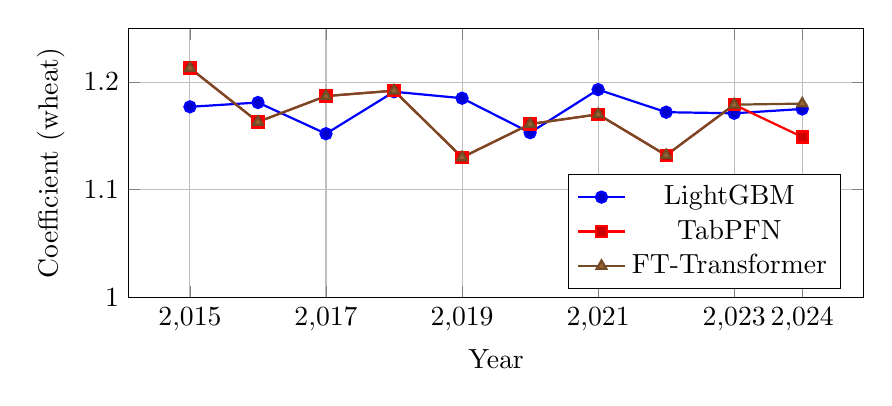
\begin{tikzpicture}
\begin{axis}[
  width=0.9\linewidth,
  height=5cm,
  xlabel={Year},
  ylabel={Coefficient (wheat)},
  ymin=1.0, ymax=1.25,
  xtick={2015,2017,2019,2021,2023,2024},
  legend pos=south east,
  grid=both,
]
\addplot+[mark=*, thick] coordinates {(2015,1.177) (2016,1.181) (2017,1.152) (2018,1.191) (2019,1.185) (2020,1.153) (2021,1.193) (2022,1.172) (2023,1.171) (2024,1.175)};
\addlegendentry{LightGBM}
\addplot+[mark=square*, thick] coordinates {(2015,1.213) (2016,1.163) (2017,1.187) (2018,1.192) (2019,1.130) (2020,1.161) (2021,1.170) (2022,1.132) (2023,1.179) (2024,1.149)};
\addlegendentry{TabPFN}
\addplot+[mark=triangle*, thick] coordinates {(2015,1.213) (2016,1.163) (2017,1.187) (2018,1.192) (2019,1.130) (2020,1.161) (2021,1.170) (2022,1.132) (2023,1.179) (2024,1.18)};
\addlegendentry{FT-Transformer}
\end{axis}
\end{tikzpicture}
\caption{National wheat out-of-home consumption coefficient over time, selected models.}
\label{fig:app_wheat_trend}
\end{figure}

\begin{figure}[htbp]
\centering
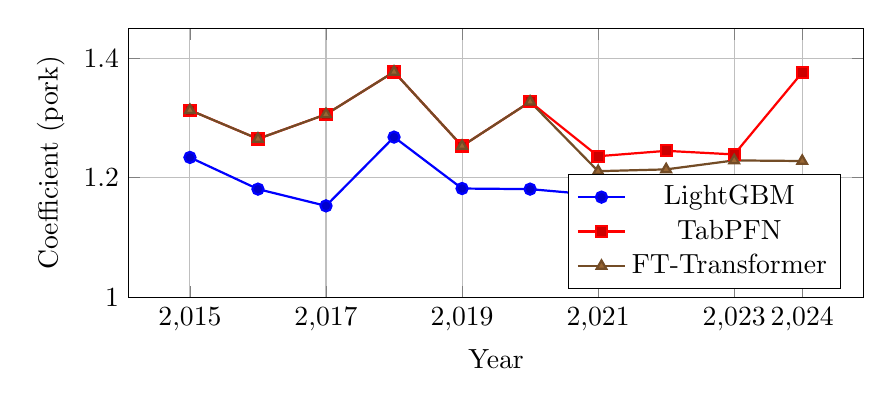
\begin{tikzpicture}
\begin{axis}[
  width=0.9\linewidth,
  height=5cm,
  xlabel={Year},
  ylabel={Coefficient (pork)},
  ymin=1.0, ymax=1.45,
  xtick={2015,2017,2019,2021,2023,2024},
  legend pos=south east,
  grid=both,
]
\addplot+[mark=*, thick] coordinates {(2015,1.234) (2016,1.181) (2017,1.153) (2018,1.268) (2019,1.182) (2020,1.181) (2021,1.171) (2022,1.159) (2023,1.164) (2024,1.168)};
\addlegendentry{LightGBM}
\addplot+[mark=square*, thick] coordinates {(2015,1.313) (2016,1.265) (2017,1.306) (2018,1.377) (2019,1.253) (2020,1.327) (2021,1.236) (2022,1.245) (2023,1.239) (2024,1.376)};
\addlegendentry{TabPFN}
\addplot+[mark=triangle*, thick] coordinates {(2015,1.313) (2016,1.265) (2017,1.306) (2018,1.377) (2019,1.253) (2020,1.327) (2021,1.211) (2022,1.214) (2023,1.229) (2024,1.228)};
\addlegendentry{FT-Transformer}
\end{axis}
\end{tikzpicture}
\caption{National pork out-of-home consumption coefficient over time, selected models.}
\label{fig:app_pork_trend}
\end{figure}

\section*{References}
\addcontentsline{toc}{section}{References}

\bibliographystyle{apalike}
\bibliography{references}

\end{document}

